\chapter{Inverse Kinematics}
\label{chap:inv kin}


\section{Introduction}

The goal of the robotics project is to control the movement of a 7 DOF robot arm with several joints. This is being done by controlling the different joint positions based on the required robot arm positions for the execution of a specific task. A Baxter robot is used for this project and the chosen task to execute is the painting of a circle. 


\section{Denavit-Hartenberg parameters}
\subsection{Theoretical calculation}
To be able to compute the inverse kinematics of a robot efficiently in a minimal and systematic way, the kinematics of the system can be described using Denavit-Hartenberg parameters. \\
Before doing this, it is important to note that Baxter has seven joints for each arm (which means 7 degrees of freedom) while a task in the real world 3D space needs only six degrees of freedom, namely three rotations and three translations. Therefore, the arms of Baxter have one redundant degree of freedom for general tasks.\\
Redundancy can be helpful for avoiding obstacles, increasing the range of the workspace or allow to reach a position and orientation by avoiding it (which increases the complexity of the control).\\
The group has chosen in this case to fix a joint, $E_0$ not represented in the Figure (\ref{fig:DHparam}) but present on the information on Baxter website.\footnote{\url{http://sdk.rethinkrobotics.com/wiki/Hardware\_Specifications}} The reason for this will become clear in section \ref{sec: inv}.\\

\noindent The first thing to do to calculate the DH parameters is to fix the frame of each joint. Some rules have to be respected: \\
\begin{itemize}
\item $z_{i-1}$ axis has to be along the axis of joint i
\item $x_{i-1}$ axis is along the common normal between joint axis i-1 and i
\end{itemize}

\noindent The origin is simply on the intersection of x and z and the y-axis can be found thanks to the right-hand rule.\\
\newpage

However some specific cases still have to be defined: \\
\begin{itemize}
\item the origin and the $x_0$-axis are chosen freely
\item the $z_n$-axis is not specified (but $x_n$ must be orthogonal to and intersect $z_{n-1}$)
\item if $z_i$ and $z_{i-1}$ are parallel, the common normal is not unique and then the origin $O_i$ can be chosen arbitrarily.
\item if $z_i$ and $z_{i-1}$ are incident, the positive direction of $x_i$ can be chosen arbitrarily (however, it is often chosen so that $x_i = z_i$ x $z_{i-1}$)
\end{itemize}

 \begin{figure}[!ht]
	\centering
    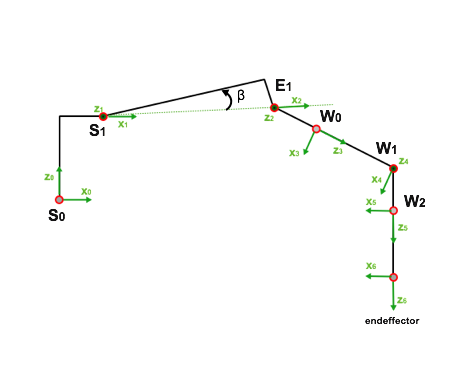
\includegraphics[width = 0.7\textwidth]{Images/DHparam2}
    \caption{Schematic drawing of the Baxter arm for the determination of the DH parameters.}
    \label{fig:DHparam}
\end{figure}

\noindent The frames are now fixed, the DH parameters can then be calculated according to the following convention rules :\\
\begin{itemize}
\item $a_i$ is the distance between the two points that intersect the joint axis $z_i$ and $z_{i+1}$ with their common normal
\item $d_i$ is the distance between the origin $O_i$ and the intersection between the joint axis $z_i$ and the common normal with joint axis $z_{i+1}$
\item $\alpha_i$ is the twist angle between the joint axis $z_i$ and $z_{i+1}$
\item $\theta_i$ is the joint angle between $x_{i-1}$ and $x_i$ around $z_{i-1}$
\end{itemize}

\noindent A summary of the determination of these parameters coming from the course.\footnote{Course of robotics of Michael Van Damme}:

\vspace{1cm}

\begin{figure}[!h]
	\centering
    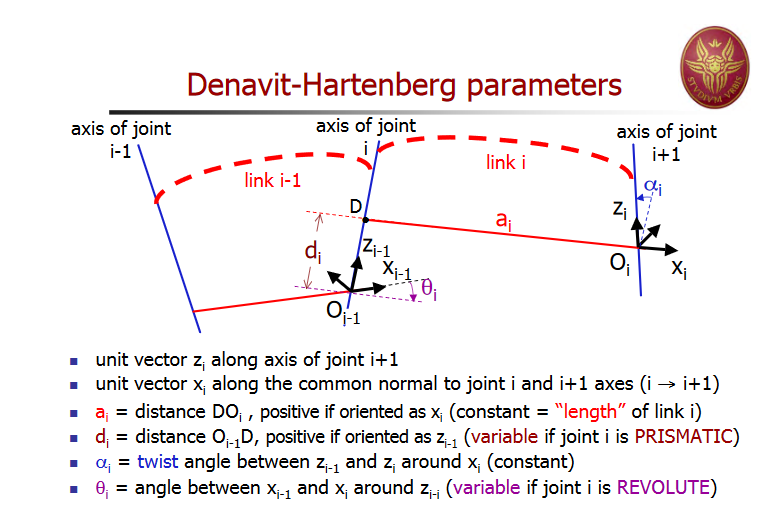
\includegraphics[width = 0.9\textwidth]{Images/DHparameters}
    \caption{Determination of DH parameters}
    \label{fig:DH}
\end{figure}

\noindent These parameters allow the calculation of the matrix defining the roto-translation around and along $x_{i-1}$ and $z_{i-1}$. \\

\begin{center}
	\begin{equation}
		A^{i-1}_{i}(q_i) = A^{i-1}_{i'}(q_i) * A^{i'}_{i}(q_i) = \begin{bmatrix}
		c\theta_i & -c\alpha_is\theta_i & s\alpha_is\theta_i & a_ic\theta_i \\
        s\theta_i & c\alpha_ic\theta_i & -s\alpha_ic\theta_i & a_is\theta_i \\
        0 & s \alpha_i & c \alpha_i & d_i\\
        0 & 0 & 0 & 1
		\end{bmatrix}
	\end{equation}
\end{center}


\noindent The matrix of a roto-translation can be represent as: \\
\begin{center}
	 \begin{equation}
	 	T^i_{i-1} = \begin{bmatrix}
	 	R & p\\ 0 & 1
	 	\end{bmatrix}
	 \end{equation}
\end{center}

\noindent where R is a 3x3 matrix of rotation, p is a 3x1 vector representing the translation between $O_{i-1}$ and $O_i$, 0 is a 1x3 null matrix and 1 is simply a scalar.

\subsection{Results of DH parameters}

The obtained values for the DH parameters are represented in the following table.\\

\begin{center}
	\begin{tabular}{c|c c c c }

		Joint & $a_i$ & $d_i$ & $\alpha_i$  & $\theta_i$ \\
        \hline
        $S_0$ & 69 & 270.35 & $\pi$ /2 & $\theta_1$ \\
        $S_1$ & 370.82 & 0 & 0 & $\theta_2$ + $\beta$\\
        $E_1$ & 0 & 0 & - $\pi$/2 & $\theta_3$ + $\pi$ + $\beta$\\
        $W_0$ & 10 & 374.29 & $\pi/2$ & $\theta_4$\\
        $W_1$ & 0 & 0 & - $\pi$ /2 & $\theta_5$ \\
        $W_2$ & 0 & 229.525 & 0 & $\theta_6$
	\end{tabular}
\end{center}

\noindent where $\beta$ is $arctan(\frac{69}{364.35})$ or $10,7^\circ$ (see Figure \ref{fig:DHparam}).


\section{Task Description}
The calculations for the inverse kinematics can be simplified based on the tasks that will have to be executed. This will allow to fix some degrees of freedom, or some relationships between the joint angles.\\
\noindent The task that the robot will execute is the following: the robot will pick a paint brush, dip it in a cup with some acrylic paint, draw a circle on a sheet of paper and then place the brush in a cup of water. To calibrate the orientation of the paper sheet at the beginning of the execution, the robot arm will first point to two reference points, which will have to correspond to those shown in Figure \ref{fig:Task}. The robot will then bring the brush to the consecutive waypoints, which all have their specific coordinates.


\begin{figure}[!ht]
	\centering
    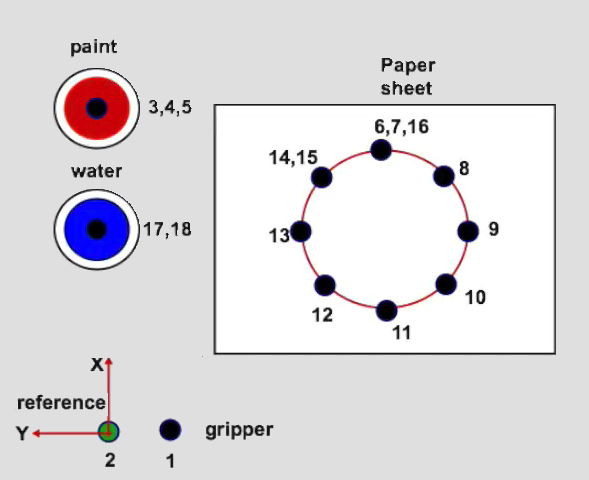
\includegraphics[width = 0.55\textwidth]{Images/Task_final}
    \caption{Projection of the waypoints describing the task on the X-Y plane, which corresponds to the table surface.}
    \label{fig:Task}
\end{figure}

\bigskip
\noindent A first observation is that the last link in the kinematic chain can stay in a vertical position during the whole execution process. Also, the paint brush does not have to rotate around the vertical axis, so that joint W2 can be fixed. Since it is assumed that there are no specific constrains for the workspace of the robot arm, there are still some redundant degrees of freedom that will not be used. Therefore, joint W0 can also be fixed. Further developments will be discussed.


\section{Inverse kinematics}
\label{sec: inv}
The equations for the inverse kinematics can be complicated so the group has tried to simplify them as much as possible.\\
The six remaining joints of the robot can be divided in two parts. The three last joint correspond to a spherical wrist and so will focus on the orientation of the end-effector while the three other joints will be used to put the end-effector at the right position.\\

\noindent As the task that will have to be executed by the robot is a paint drawing, the paintbrush can be perpendicular to the table. So the joint $W_0$ can be fixed to 0 and the joint $W_1$ has to compensate joint $S_1$ and $E_1$ so that $z_5$ is parallel to $z_0$. The $90^{\circ}$ between $S_1$ and $E_1$ has to be taken into account. Another important consideration which serves as a reference is that if the angles of all the joints are set to zero, the arm stretches horizontally.\\
It is now easy to see than $\theta_5 = \pi /2 - (\theta_1 + \theta_2)$. \\
The last joint has no importance in our case and has been fixed arbitrarily to zero.\\

\noindent The position of the robot still has to be calculated. The position of the end-effector will be evaluated based on the wrist centerpoint and the rotation between the first and the last frames. \\

\begin{center}
	\begin{equation}
		p^0_e = p^0_w + d_6 z ^0_6 = p^0_w + d_6 R_e^0 \begin{vmatrix}
		0 \\ 0 \\ 1
		\end{vmatrix}
	\end{equation}
\end{center}

\begin{center}
	\begin{equation}
		p^0_w = p^0_e - d_6 R_e^0 \begin{vmatrix}
		0 \\ 0 \\ 1
		\end{vmatrix}
	\end{equation}
\end{center}

\noindent Where $d_6^0$ is the distance between the wrist centerpoint and the end-effector and $R^0_e$ is the rotation between frame 0 and frame 6 that is equivalent to a rotation of 180$^\circ$ around the y-axis of one of these two frames. The arm being perpendicular to the table, the difference between the wrist centerpoint and the end-effector is simply a difference of height that correspond to 270.35 - 229.525. \\


\noindent For the calculation of the position to reach, the raisonning looks like one example made during the course. The angle $\theta1$ corresponds to the orientation of the arm. It is calculated thanks to the x and y that will be given using the equation of trigonometry.\\

\begin{center}
	\begin{equation}
		\theta_1 = Atan2(y_c,x_c)
	\end{equation}
\end{center}

\noindent The function Atan2 allows to have an angle between - $\pi$ and $\pi$ instead of between 0 and $\pi$.\\

\noindent The two last angles are slightly more difficult to calculate.\\

\begin{figure}[!ht]
	\centering
    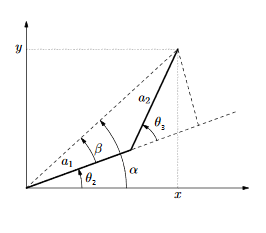
\includegraphics[width = 0.6\textwidth]{Images/angles}
    \caption{Calculation of $\theta_2$ and $\theta_3$}
    \label{fig:angles}
\end{figure}

\noindent The angle $\pi - \theta_3$ is found thanks to the Pythagore formula.\\

\begin{center}
	\begin{equation}
		x^2 + y^2 = a_1^2 + a_2^2 - 2a_1a_2cos(\pi - \theta_3) = a_1^2 + a_2^2 + 2a_1a_2cos(\theta_3)
	\end{equation}
\end{center}

\begin{center}
	\begin{equation}
		cos(\theta_3) = \frac{x^2 + y^2 - a_1^2 - a_2^2}{2a_1a_2}
	\end{equation}
\end{center}

\noindent To be able to use the function Atan2, the sine of the angle is also need:\\

\begin{center}
	\begin{equation}
		sin(\theta_3) = \sqrt{1 - (cos(\theta_3))^2}
	\end{equation}
\end{center}

\noindent So that: 

\begin{center}
	\begin{equation}
		\theta_3 = Atan2(sin(\theta_3),cos(\theta_3))
	\end{equation}
\end{center}

\noindent The base of the calculation is $\theta_2$ equals $\alpha$ minus $\beta$.\\
The calculation of $\alpha$ is the same than for $\theta_1$ and the calculation of $\beta$ is made thanks to the triangle in dashed line.

\begin{center}
	\begin{equation}
		tg(\beta) = \frac{a_2sin(\theta_3)}{a_1+a_2 cos(\theta_3)}
	\end{equation}
\end{center}

\noindent So that $\theta_2$ can be obtained as follows:

\begin{center}
	\begin{equation}
		\theta_2 = Atan2(y,x) - Atan2(a_2sin(\theta_3),a_1+a_2 cos(\theta_3))
	\end{equation}
\end{center}